\section{Results}
\label{sec:results}

\subsection{Main table (35 backbones, 5,936 designs)}
\label{sec:main-table}

% Figure numbers follow the numbering assigned in the markdown source
% (Figure 2 appears in Section 4.1, Figure 1 in Section 4.2). The counters
% are set explicitly so that the compiled paper keeps the same number for
% each figure.
\setcounter{figure}{1}

\begin{table*}[htbp]
  \centering
  \scriptsize
  \setlength{\tabcolsep}{2pt}
  \begin{tabular}{@{}lrrrrrrrr@{}}
    \toprule
    Arm & n & surface apolar & aggregation 5-mer & net charge & pI & recovery & diversity & \textbf{scTM} \\
    \midrule
    ProteinMPNN & 560 & 0.430 & 0.212 & $+1.95$ & 7.87 & 0.436 & 0.283 & 0.8444 \\
    ProteinMPNN (seed 1) & 560 & 0.434 & 0.212 & $+1.89$ & 7.82 & 0.437 & 0.288 & 0.8434 \\
    SolubleMPNN & 560 & 0.378 & 0.168 & $-1.57$ & 6.64 & 0.425 & 0.283 & 0.8457 \\
    HyperMPNN & 560 & 0.411 & 0.213 & $+4.30$ & 8.40 & $\bm{0.376}$ & 0.258 & $\bm{0.7809}$ \\
    MembraneMPNN (global) & 528 & 0.376 & 0.178 & $+0.30$ & 7.49 & 0.439 & 0.288 & 0.8748 \\
    LigandMPNN & 528 & 0.397 & 0.176 & $-1.00$ & 6.64 & 0.443 & 0.263 & 0.8717 \\
    guide surf $\lambda$10 & 528 & $\bm{0.259}$ & 0.120 & $+1.72$ & 7.87 & 0.446 & 0.272 & 0.8703 \\
    guide agg $\lambda$10 & 528 & 0.291 & $\bm{0.124}$ & $\bm{+1.96}$ & 7.97 & 0.448 & 0.280 & $\bm{0.8718}$ \\
    guide charge $\lambda{+}3$ & 528 & 0.413 & 0.206 & $\bm{-8.52}$ & 5.35 & 0.456 & 0.277 & 0.8618 \\
    guide surf10/charge$-2$ & 528 & 0.250 & 0.112 & $\bm{+12.83}$ & 9.94 & 0.444 & 0.276 & 0.8726 \\
    guide surf10/charge$+2$ & 528 & 0.258 & 0.120 & $\bm{-8.70}$ & 5.57 & 0.448 & 0.266 & 0.8671 \\
    \bottomrule
  \end{tabular}
  \caption{Main table (35 backbones, 5{,}936 designs).}
  \label{tab:main}
\end{table*}

Folded backbones per arm: 35 for ProteinMPNN/SolubleMPNN/HyperMPNN, 33 for
MembraneMPNN/LigandMPNN and the guided arms (two backbones failed to sample for
those arms). All comparisons are paired, so the differing counts do not affect
the intervals.

\paragraph{Repeatability.}
Seed 0 $\to$ seed 1, same weights and temperature: $\Delta$scTM =
$\bm{-0.0010}$, 95\% CI $[-0.0086, +0.0076]$ (35 backbones). This $\pm 0.008$
band is the resolution floor of the benchmark and the reason every comparison
below is paired.

\begin{table*}[htbp]
  \centering
  \scriptsize
  \setlength{\tabcolsep}{2pt}
  \begin{tabular}{@{}lllllp{1.0in}l@{}}
    \toprule
    Arm & $\Delta$scTM & CI & $p$ (raw) & $p$ (Holm) & targeted change & leakage \\
    \midrule
    SolubleMPNN & $+0.0013$ & $[-0.0118, +0.0169]$ & 0.89 & 1.00 & surface $-12.1$\% & charge $-3.5$ \\
    \textbf{HyperMPNN} & $\bm{-0.0635}$ & $\bm{[-0.1259, -0.0117]}$ & $\bm{0.006}$ & $\bm{0.057}$ & surface $-4.4$\% & charge $+2.4$ \\
    MembraneMPNN (global) & $+0.0207$ & $[-0.0013, +0.0561]$ & 0.096 & 0.76 & surface $-12.6$\% & charge $-1.7$ \\
    LigandMPNN & $+0.0176$ & $[-0.0033, +0.0513]$ & 0.21 & 1.00 & surface $-7.7$\% & charge $-3.0$ \\
    \textbf{guide surf $\lambda$10} & $+0.0066$ & $[-0.0054, +0.0215]$ & 0.34 & 1.00 & surface $\bm{-39.8\%}$ & charge $-0.2$ \\
    \textbf{guide agg $\lambda$10} & $+0.0081$ & $[-0.0020, +0.0216]$ & 0.16 & 1.00 & aggregation $\bm{-42\%}$ & charge 0.0 \\
    guide charge $\lambda{+}3$ & $-0.0019$ & $[-0.0100, +0.0069]$ & 0.63 & 1.00 & charge $\bm{-10.5}$ & surface $-4.0$\% \\
    guide surf10/charge$-2$ & $+0.0089$ & $[-0.0057, +0.0278]$ & 0.30 & 1.00 & surface $-41.9$\%, \newline charge $+10.9$ & --- \\
    guide surf10/charge$+2$ & $+0.0034$ & $[-0.0116, +0.0219]$ & 0.74 & 1.00 & surface $-40.0$\%, \newline charge $-10.7$ & --- \\
    \bottomrule
  \end{tabular}
  \caption{Paired cost of control (vs ProteinMPNN, 95\% bootstrap CI over
  backbones).}
  \label{tab:paired-cost}
\end{table*}

\paragraph{What ``zero cost'' means quantitatively.}
The paired upper 95\% confidence limits of the five guided arms are $+0.007$ to
$+0.028$ scTM. We can therefore exclude a foldability cost larger than
\textbf{0.03 scTM (about 3.5\% relative)} for any guided arm, while their point
estimates run \emph{above} the baseline. ``Zero cost'' is shorthand for that
bound, not for a null effect.

\paragraph{Diversity is matched and does not explain the result.}
Across the ten arms the measured diversity spans only 0.256 to 0.292, and it
correlates \emph{positively} with scTM ($r = +0.61$ across arms): the arms that
fold better are also the more diverse ones, so no arm is buying quality with
diversity. Comparisons are therefore already at matched diversity and an
explicit S@D curve would not change the ordering.

\paragraph{Multiple comparisons matter here.}
With ten arms and therefore nine comparisons against one baseline, one CI
excludes zero before correction and \textbf{none survives Holm} (HyperMPNN raw
$p = 0.006$, Holm $p = 0.057$; MembraneMPNN, which excluded zero at 8 designs per
cell, does not at 16, raw $p = 0.096$). We therefore read these as effects of
interest rather than confirmed differences, and the same rule is applied
everywhere in this paper.

With that caveat the pattern is still clear. \textbf{HyperMPNN}, the thermophile-retrained model, carries the only negative point estimate of any arm:
$\bm{-0.0635}$ scTM (CI $[-0.1259, -0.0117]$) and a 14\% relative recovery loss
for a 4.4\% surface reduction. \textbf{MembraneMPNN(global)} --- conditioning on
a label rather than retraining --- has the largest positive estimate
($+0.0207$), although its interval now contains zero.
The guided arms move the target property 3--9$\times$ further than any published
model \textbf{and} stay on the zero-cost line.

The honest reading is a \textbf{trade-off in the arm family, not a proven
winner}: retraining buys the least property movement per unit of quality risk,
conditioning buys a little with no risk, and closed-form guidance buys the most
with no measurable risk. Only the last comparison is large enough to be
insensitive to correction.

\begin{figure*}[htbp]
  \centering
  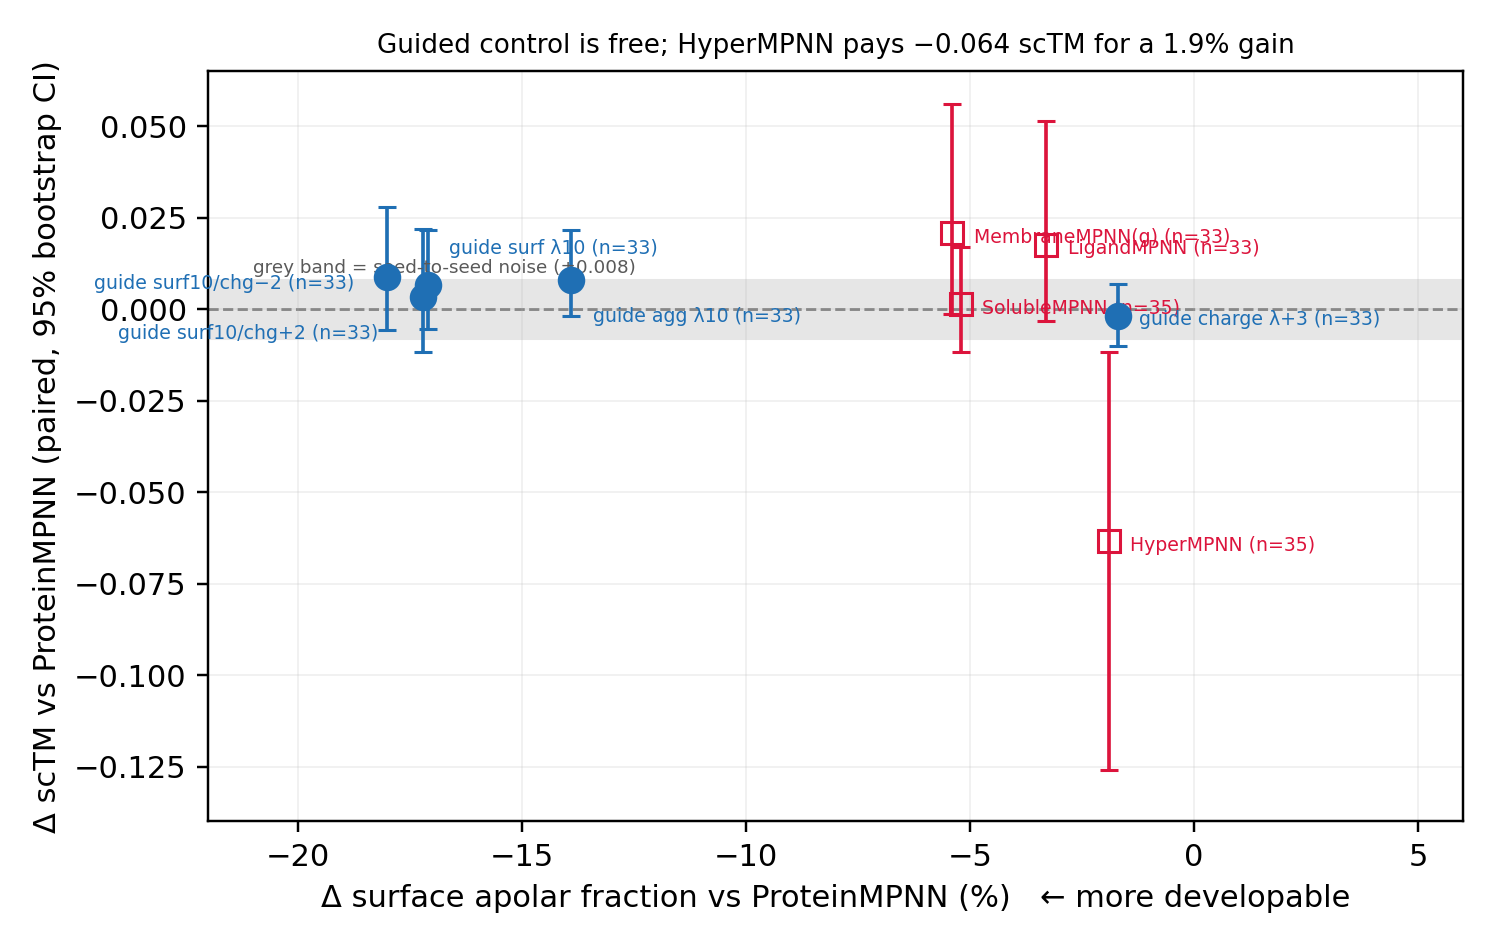
\includegraphics[width=0.62\linewidth]{figs/fig2_property_vs_sctm.png}
  \caption{Paired $\Delta$scTM versus $\Delta$ surface hydrophobicity. Grey
  band: reproducible seed-to-seed noise ($\pm 0.008$). All arms sit on the
  zero-cost line; guided arms (blue) move three times further left than
  published models (red).}
  \label{fig:property-vs-sctm}
\end{figure*}

\subsection*{4.1b Diversity is the real axis, and guidance moves the whole curve}
\label{sec:diversity-temperature}

Table~\ref{tab:main} sits at one temperature. Re-running the surface-guided arm
at $T = 0.3$ (33 backbones, 8 designs per cell, 264 folds;
Table~\ref{tab:temperature}) raises diversity from 0.277 to \textbf{0.390} ---
the same direction ProteinMPNN moves with temperature --- and simultaneously lets
guidance reach \textbf{$\bm{-70}$\% surface apolar and $\bm{-59}$\%
aggregation}. The paired cost of moving from $T{=}0.1$ to $T{=}0.3$ inside the
arm is $\Delta$scTM = $-0.0114$ (95\% CI $[-0.0228, +0.0016]$).

That is a genuine quality-diversity trade \textbf{within} the arm, and it makes
the comparison unambiguous: at $T{=}0.3$ the guided design set has
\textbf{higher diversity than the unguided baseline and higher scTM at once}
(0.390 and 0.8608 against 0.278 and 0.8434). For a model family where diversity
is a control variable rather than a nuisance, this is why we report the
(diversity, scTM, property) surface instead of a single operating point.

\subsection{Two properties, independently controlled}
\label{sec:control-plane}

On a 7-backbone pilot ($3\times3$ grid of surface
$\lambda \in \{0,5,10\}$ $\times$ charge $\lambda \in \{-2,0,+2\}$, 432 designs,
432 folds):

The full $3\times3$ grid of achieved (surface apolar, net charge) pairs is in
Table~\ref{tab:control-plane}; scTM across the whole plane stays in
0.9229--0.9348. Rows are nearly horizontal and columns nearly vertical: the two
axes are close to orthogonal. Table~\ref{tab:main} reproduces this
(surf10/charge$-2$ vs surf10/charge$+2$: surface 0.250 vs 0.258, charge $+12.83$
vs $-8.70$).

\setcounter{figure}{0}
\begin{figure*}[htbp]
  \centering
  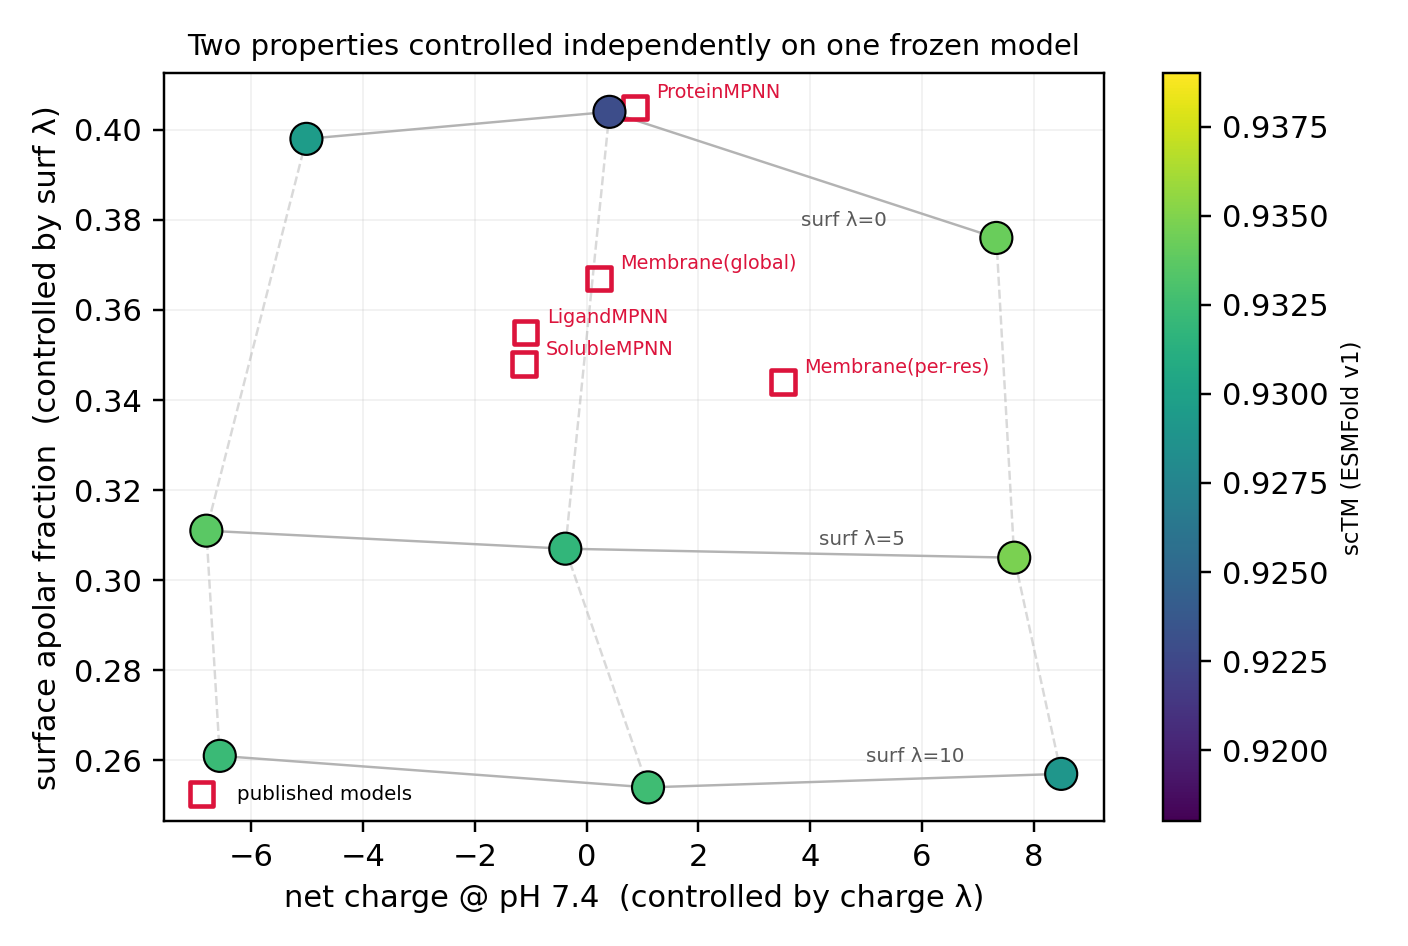
\includegraphics[width=0.62\linewidth]{figs/fig1_control_plane.png}
  \caption{The $3\times3$ control plane (filled circles, coloured by scTM)
  versus published models (open red squares), each of which is a single point.}
  \label{fig:control-plane}
\end{figure*}

\subsection{Controllability slope and leakage}
\label{sec:slope-leakage}

The slope \emph{k} is measured on the full benchmark, not a pilot. We swept the
surface objective over $\lambda \in \{2, 5, 10, 20\}$ with 16 designs per cell on
all 35 backbones (560 designs per $\lambda$, 2,240 designs, all folded):

\begin{table*}[htbp]
  \centering
  \footnotesize
  \setlength{\tabcolsep}{2pt}
  \begin{tabular}{@{}lrrrrr@{}}
    \toprule
    $\lambda$ & surface apolar & aggregation 5-mer & net charge & scTM & $\Delta$scTM vs ProteinMPNN [95\% CI] \\
    \midrule
    2 & 0.368 & 0.171 & $+2.08$ & 0.8472 & $+0.0028$ $[-0.0006, +0.0067]$ \\
    5 & 0.308 & 0.136 & $+1.60$ & 0.8472 & $+0.0028$ $[-0.0054, +0.0123]$ \\
    10 & 0.253 & 0.114 & $+1.52$ & 0.8507 & $+0.0062$ $[-0.0051, +0.0207]$ \\
    20 & $\bm{0.178}$ & 0.094 & $+1.74$ & 0.8471 & $+0.0027$ $[-0.0133, +0.0218]$ \\
    \bottomrule
  \end{tabular}
  \caption{Surface-objective sweep on the full benchmark ($\lambda \in \{2,5,10,20\}$,
  16 designs per cell, 35 backbones).}
  \label{tab:lambda-sweep}
\end{table*}

Fitting a line per backbone (OLS over the four $\lambda$ values) and averaging
over backbones gives \textbf{$k_{\mathrm{surface}} = \bm{-0.01005}$
surface-apolar fraction per $\lambda$ unit}, 95\% bootstrap CI
$[-0.01113, -0.00905]$, with mean per-backbone $R^2 = \bm{0.940}$ and a usable
fit on 35 of 35 backbones. One $\lambda$ unit therefore buys about one
percentage point of surface apolarity, and the relation is linear over a
factor-of-ten range of control strength: $\lambda{=}20$ reaches 0.178, a
\textbf{58.6\% relative reduction} from the ProteinMPNN baseline of 0.430.

The corresponding slope for foldability is
\textbf{$k_{\mathrm{scTM}} = \bm{+0.00001}$ scTM per $\lambda$ unit} (CI
$[-0.00072, +0.00083]$, $p = 0.98$). Foldability is flat across the entire
sweep, and no arm's interval at any $\lambda$ excludes zero. This is the
quantitative form of ``control is free'': not that one operating point happens
to be cheap, but that the cost stays flat while the targeted property moves by a
factor of two.

\textbf{The exposure mask is load-bearing.} A control experiment at
$\lambda{=}20$ applies the same apolar penalty to \emph{all} positions instead
of only the less-buried half. It controls the target somewhat better (surface
0.159 vs 0.178, paired $\Delta = -0.019$; aggregation 0.028 vs 0.094) but pays
for it: \textbf{$\Delta$scTM = $\bm{-0.0325}$} against the masked arm (95\% CI
$[-0.0748, -0.0019]$, $p = 0.028$), and it leaks composition (net charge +3.28
vs +1.74, pI 8.29 vs 7.96). The position-specific part of the reward is
therefore what keeps control from damaging foldability, and a benchmark that
only measured the targeted property would have scored the worse method as
better.

\textbf{Leakage is a property of the reward's weight vector, not of the model.}
Kyte--Doolittle assigns negative weights to K and R, so optimising GRAVY
necessarily loads positive charge: at $\lambda{=}4$ on the pilot set, GRAVY is
$-1.63$ with net charge $+9.6$ and pI 9.8, while scTM stays at 0.926. The
aggregation reward, whose weight vector is nearly orthogonal to charge, leaks
0.0 units. Surface targeting leaks into aggregation monotonically (0.171 $\to$
0.094 across the sweep) because the two penalties share the apolar residue set,
but leaves charge and pI near the baseline.

\setcounter{figure}{2}
\begin{figure*}[htbp]
  \centering
  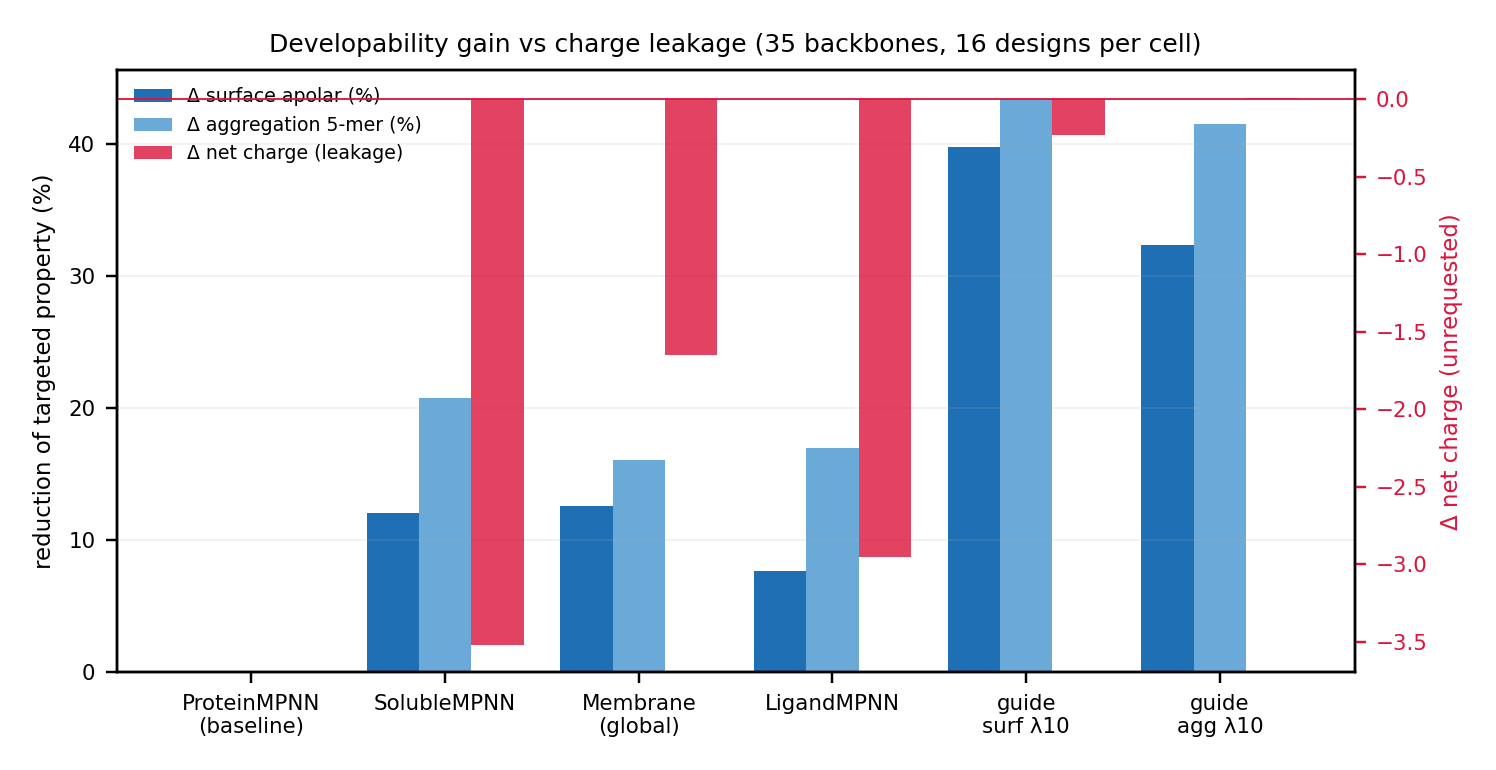
\includegraphics[width=0.62\linewidth]{figs/fig3_leakage.png}
  \caption{Targeted gain versus charge leakage for the four published arms plus the
  two surface/aggregation guided arms. Published models leak 1.7 to 3.5 charge
  units for a 4 to 13\% surface gain; the aggregation arm leaks 0.0 for a 42\%
  aggregation gain.}
  \label{fig:leakage}
\end{figure*}

\subsection{Oracle agreement: the conclusion holds, the ranking does not}
\label{sec:oracle}

We refolded 9 arms $\times$ 6 backbones $\times$ 2 designs (108 requested, 104 folded) with
\textbf{Protenix-2}~\cite{protenix} in single-sequence mode
(\texttt{--use\_msa False}), an architecture unrelated to
ESMFold~\cite{esmfold}.

Per-arm values for both oracles are in Table~\ref{tab:oracle}. Three observations:
Three observations:
\begin{enumerate}
\item \textbf{Absolute scale differs by 0.15} (ESMFold $\approx$0.93,
  single-sequence Protenix $\approx$0.72--0.81), so scTM is not comparable
  across oracles.
\item \textbf{Arm ranking is essentially unrelated}: Spearman across the 9 arms
  = $\bm{-0.18}$ ($p = 0.64$) --- the two oracles do not rank the arms
  consistently on this subset.
\item \textbf{The claim survives}: under Protenix \emph{every} arm beats
  vanilla ($+0.01$ to $+0.08$), with the two guidance arms on top; under
  ESMFold every arm is within $\pm 0.008$ of vanilla. ``Control does not cost
  foldability'' is oracle-robust even though ``which arm is best'' is not.
\end{enumerate}

Per-design correlation between the two oracles is \textbf{negative}
($n = 98$, Pearson $-0.45$, Spearman $-0.48$): ESMFold's scores are compressed
at the 0.92--0.94 ceiling, so its residual ordering is noise dominated.

\emph{Caveat.} The Protenix run is single-sequence (no MSA), a deliberately
cheap and degraded usage; it is used only to test direction, not to rank.

\subsection*{4.5 Per-backbone heterogeneity: arm means hide bimodal failure}
\label{sec:heterogeneity}

Averaging over 35 backbones is a lossy summary, and the loss matters here.

(Per-arm medians, means and worst-case collapses are in
Table~\ref{tab:heterogeneity}; the paragraphs below use them.)


HyperMPNN is the clearest case. On the \textbf{median backbone it differs from
ProteinMPNN by $\bm{-0.005}$}, and 26 of 35 backbones sit within $\pm 0.05$. But
three backbones collapse completely: 1SRL 0.220 vs 0.773, 1TIT 0.230 vs 0.862,
3PGK 0.164 vs 0.756. The mean $-0.064$ is therefore not ``a small uniform loss'';
it is \textbf{no change on most backbones plus catastrophic failure on 3 of 35},
and removing those three collapses brings the mean to $-0.014$. These are not
degenerate samples: all sixteen designs per cell are unique and their composition
entropy (3.3--4.0 bits) is indistinguishable from ProteinMPNN on the same
backbones, so the collapse is a property of the thermophile-trained prior on
these folds, not a sampling artefact.

Two consequences for benchmarking. First, \textbf{a per-arm mean is the wrong
summary statistic} for a model family where failure is bimodal; a benchmark
should report the per-backbone tail, which is why we release the full
$35 \times 10$ matrix (\texttt{results/b30\_designs.tsv}) instead of only the
aggregate. Second, \textbf{half of this benchmark has no discriminating power}:
13 of 35 backbones score above 0.92 for every arm with an arm-to-arm spread of
0.01--0.03, so any conclusion about arm differences comes from the roughly 15
backbones below 0.92.

The guided arms are the flattest: their median per-backbone change is
$\leq 0.002$ and their worst case is 0.18, an order of magnitude smaller than
the retrained or conditioned models. Whatever the guidance does, it does it
evenly.
